\begin{figure}[t]
\centering\footnotesize
\resizebox{\columnwidth}{!}{%
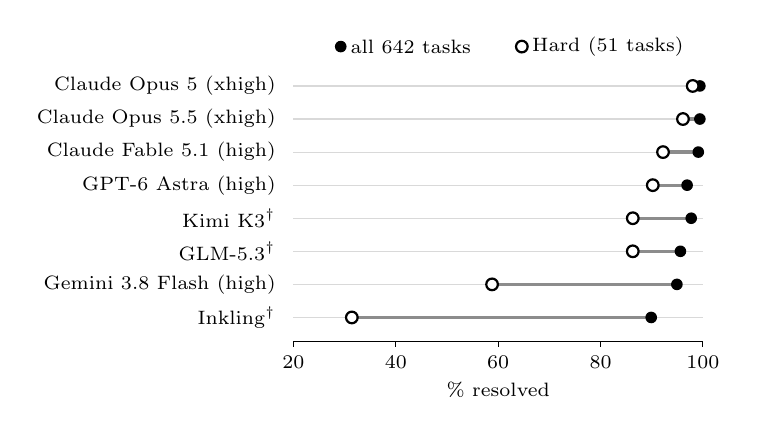
\begin{tikzpicture}
\node[anchor=east,font=\scriptsize] at (-0.1,0.00) {Claude Opus 5 (xhigh)};
\draw[gray!30] (0,0.00) -- (5.2,0.00);
\draw[line width=1.2pt,black!45] (5.070,0.00) -- (5.161,0.00);
\fill[black] (5.161,0.00) circle (2.1pt);
\draw[black,fill=white,line width=0.8pt] (5.070,0.00) circle (2.1pt);
\node[anchor=east,font=\scriptsize] at (-0.1,-0.42) {Claude Opus 5.5 (xhigh)};
\draw[gray!30] (0,-0.42) -- (5.2,-0.42);
\draw[line width=1.2pt,black!45] (4.946,-0.42) -- (5.161,-0.42);
\fill[black] (5.161,-0.42) circle (2.1pt);
\draw[black,fill=white,line width=0.8pt] (4.946,-0.42) circle (2.1pt);
\node[anchor=east,font=\scriptsize] at (-0.1,-0.84) {Claude Fable 5.1 (high)};
\draw[gray!30] (0,-0.84) -- (5.2,-0.84);
\draw[line width=1.2pt,black!45] (4.693,-0.84) -- (5.141,-0.84);
\fill[black] (5.141,-0.84) circle (2.1pt);
\draw[black,fill=white,line width=0.8pt] (4.693,-0.84) circle (2.1pt);
\node[anchor=east,font=\scriptsize] at (-0.1,-1.26) {GPT-6 Astra (high)};
\draw[gray!30] (0,-1.26) -- (5.2,-1.26);
\draw[line width=1.2pt,black!45] (4.563,-1.26) -- (4.999,-1.26);
\fill[black] (4.999,-1.26) circle (2.1pt);
\draw[black,fill=white,line width=0.8pt] (4.563,-1.26) circle (2.1pt);
\node[anchor=east,font=\scriptsize] at (-0.1,-1.68) {Kimi K3$^\dagger$};
\draw[gray!30] (0,-1.68) -- (5.2,-1.68);
\draw[line width=1.2pt,black!45] (4.309,-1.68) -- (5.051,-1.68);
\fill[black] (5.051,-1.68) circle (2.1pt);
\draw[black,fill=white,line width=0.8pt] (4.309,-1.68) circle (2.1pt);
\node[anchor=east,font=\scriptsize] at (-0.1,-2.10) {GLM-5.3$^\dagger$};
\draw[gray!30] (0,-2.10) -- (5.2,-2.10);
\draw[line width=1.2pt,black!45] (4.309,-2.10) -- (4.914,-2.10);
\fill[black] (4.914,-2.10) circle (2.1pt);
\draw[black,fill=white,line width=0.8pt] (4.309,-2.10) circle (2.1pt);
\node[anchor=east,font=\scriptsize] at (-0.1,-2.52) {Gemini 3.8 Flash (high)};
\draw[gray!30] (0,-2.52) -- (5.2,-2.52);
\draw[line width=1.2pt,black!45] (2.522,-2.52) -- (4.869,-2.52);
\fill[black] (4.869,-2.52) circle (2.1pt);
\draw[black,fill=white,line width=0.8pt] (2.522,-2.52) circle (2.1pt);
\node[anchor=east,font=\scriptsize] at (-0.1,-2.94) {Inkling$^\dagger$};
\draw[gray!30] (0,-2.94) -- (5.2,-2.94);
\draw[line width=1.2pt,black!45] (0.741,-2.94) -- (4.543,-2.94);
\fill[black] (4.543,-2.94) circle (2.1pt);
\draw[black,fill=white,line width=0.8pt] (0.741,-2.94) circle (2.1pt);
\draw (0,-3.24) -- (5.2,-3.24);
\draw (0.000,-3.24) -- (0.000,-3.31) node[below,font=\scriptsize] {20};
\draw (1.300,-3.24) -- (1.300,-3.31) node[below,font=\scriptsize] {40};
\draw (2.600,-3.24) -- (2.600,-3.31) node[below,font=\scriptsize] {60};
\draw (3.900,-3.24) -- (3.900,-3.31) node[below,font=\scriptsize] {80};
\draw (5.200,-3.24) -- (5.200,-3.31) node[below,font=\scriptsize] {100};
\node[font=\scriptsize] at (2.60,-3.86) {\% resolved};
\fill[black] (0.6,0.5) circle (2.1pt) node[right,font=\scriptsize] {all 642 tasks};
\draw[black,fill=white,line width=0.8pt] (2.9,0.5) circle (2.1pt) node[right,font=\scriptsize] {Hard (51 tasks)};
\end{tikzpicture}}
\caption{Percent of tasks resolved on SWE-Bench Pro V2 (filled dots) and its Hard split (open dots) under the locked protocol. The full set separates these systems by less than 10 points (89.9--99.4\%); the Hard split spreads them from 31.4\% to 98.0\%. $^\dagger$Partner runs under the same protocol (Table~\ref{tab:main}).}
\label{fig:spread}
\end{figure}
